\chapter{Untersuchung des Laufzeitverhaltens}
Die Untersuchung der Laufzeitverhaltens wurde mithilfe eines Logik-
Analysers durchgeführt. Ein Logikanalyser misst wie lange und wann
ein Pin 1 und/oder 0 ist. Die Pins, die nötig sind um diese Messungen
durchzuführen, dürfen noch nicht belegt sein. Vorteilhafterweise
besitzt die Platine zwei Ports, die noch nicht belegt sind aber
trotzdem nach draußen gelegt wurden, somit konnte der Logik-
Analyser an die Platine angeschlossen und ein kleines Modul
geschrieben werden, um diese Pins setzen und wieder löschen zu
können. Diese Operationen wurden als Makros implementiert um den
Messoverhead so gering wie möglich zu halten.
\begin{table}[htb]
\begin{center}
	\begin{tabular}{|c||c|c|}
		\hline
		\textbf{Makro} & \textbf{benötigte Takte} & \textbf{benötigte Zeit bei 16 MHz} \\ \hline \hline
		pin\_set() & 2 & 125 ns \\ \hline
		pin\_clear() & 2 & 125 ns \\ \hline
		pin\_toggle() & 4 & 250 ns \\ \hline
	\end{tabular}
	\caption{\label{pin_takte} Benötigte Takte/Zeit für Pin-Operationen}
\end{center}
\end{table}
Wie hier beschrieben sind die Zeiten für das Ausführen der Instruktion
zum setzen, löschen und umschalten von einzelnen Pins ziemlich gering.
Doch bei den Messungen insbesondere mit einem Leistungsfähigen und
sehr genauen Oszilloskop konnte herausgefunden werden, dass das eigentliche
Wechsel des Stroms am Pin verhältnismäßig langsam durchgeführt wird,
insbesondere das Abfallen des Stromes, also bei einer fallenden Flanke
benötigt ungefähr 2 us von denen allerdings, und hier liegt das Problem,
zwischen 0.5 und 1 us fälschlicherweise als ''high'' gemessen wird.
D.h. der Logikanalyser misst eine gewisse Zeitspanne einen ''falschen'' Wert.
(Er ist nicht physikalisch falsch nur logisch). Denn wenn der Strom abfällt
ist der bin schon nicht mehr gesetzt, der Logikanalyser allerdings betrachtet
dies teilweise immer noch als gesetzt.
Aufgrund dieses Umstandes als auch der Tatsache, dass das System nicht untersucht
werden kann ohne einen geringen Fußabdruck zu hinterlassen, sind die Messungen mit
einem abschätzbaren aber nicht genau vorhersagbaren Fehler im Vergleich zur
Wirklichkeit behaftet.
\section{Erste Messungen}
Durch die ersten Messungen wurde der Startpunkt für die Untersuchung der Software
festgelegt. Dafür wurde in der Hauptschleife (siehe Abb. \ref{main_loop_full}) zum einen
ein pin\_toggle() eingebaut, um die Länge einer Schleifeniteration zu messen, zum anderen
wurde die einzelnen Funktionsaufrufe in der Hauptschleife mit pin\_set() und pin\_clear()
umgeben.
\begin{figure}[htb]
 \centering
 \scalebox{0.5}{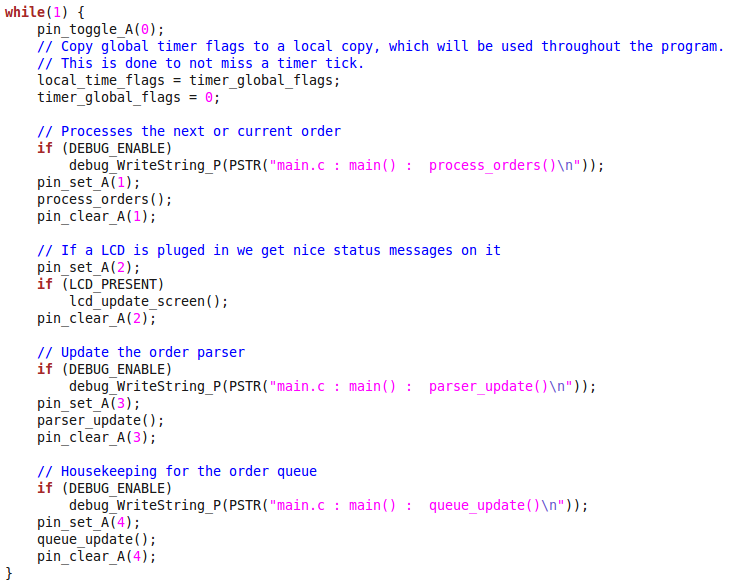
\includegraphics{pictures/main_loop_full.png}}
 \caption{\label{main_loop_full}Die Hauptschleife mit Debugausgaben und Pin-Operationen}
\end{figure}
\begin{table}[htb]
\begin{center}
	\begin{tabular}{|c||r|c|}
		\hline
		\textbf{Funktion} & \textbf{Zeit} & \textbf{Rahmenbedingungen} \\ \hline \hline
		Hauptschleife & 27,916 \textmu{}s & Idle, LCD an, DEBUG aus, I2C an, AB:EIT \\ \hline
		process\_orders() & 11,964 \textmu{}s &  \\ \hline
		lcd\_update\_screen() & 3,988 \textmu{}s &  \\ \hline
		parser\_update() & 3,988 \textmu{}s &  \\ \hline
		queue\_update() & 3,988 \textmu{}s &  \\ \hline \hline
		Hauptschleife & 47,856 \textmu{}s & ABS aktiv im Idle Status, ansonsten wie oben \\ \hline
		process\_orders() & 31,904 \textmu{}s &  \\ \hline
		lcd\_update\_screen() & 3,988 \textmu{}s &  \\ \hline
		parser\_update() & 3,988 \textmu{}s &  \\ \hline
		queue\_update() & 3,988 \textmu{}s &  \\ \hline \hline
		I2C-Bus ISR & 4,586 \textmu{}s & Adresse empfangen \\ \hline
		I2C-BUS ISR & 21,934 \textmu{}s & Daten empfangen \\ \hline
		100ms ISR & 8,076 \textmu{}s & \\ \hline \hline
		Hauptschleife & 718,843 \textmu{}s & LCD aus, Byte in Parser, Befehl bereit \\ \hline
		process\_orders() & 39,880 \textmu{}s & I2C ISR (Daten) aufgetreten \\ \hline
		lcd\_update\_screen() & 0,997 \textmu{}s &  \\ \hline
		parser\_update() & 175,474 \textmu{}s &  \\ \hline
		queue\_update() & 505,484 \textmu{}s &  \\ \hline \hline
		Hauptschleife & 3614,000 \textmu{}s & LCD an, Befehl in Queue, aber nicht gestartet \\ \hline
		process\_orders() & 358,923 \textmu{}s &  \\ \hline
		lcd\_update\_screen() & 3250,000 \textmu{}s &  \\ \hline
		parser\_update() & 6,032 \textmu{}s &  \\ \hline
		queue\_update() & 5,583 \textmu{}s &  \\ \hline
	\end{tabular}
	\caption{\label{erste_messung} Ergebnisse der ersten Messungen}
\end{center}
\end{table}
In der Tabelle \ref{erste_messung} sind die Wichtigsten Daten der ersten Messreihen zusammen
gefasst. Die Spalte ''Rahmenbedingungen'' beschreibt Bedingungen während der Messung geherrscht haben.
Hierbei bezeichnet die Bedingung ''AB:EIT'', dass das aktive Bremsen (AB:) eingeschaltet (E; Enable) ist und
sowohl aktiviert wird, wenn kein Befehl bearbeitet wird(I; Idle) oder eines der Räder seinen Trigger früher
erreicht hat als das andere (T; Trigger). ''I2C an'' bezeichnet, dass der I2C-Bus für die E/A-Operationen
verwendet wurde und nicht die UART Schnittstelle.\\
Interessant ist bei diesen Daten, dass das aktualisieren der Warteschlange, wenn ein Befehl vorliegt, gut
eine halbe millisekunde benötigt.
\section{Das LCD-Problem}
Wie in der Tabelle \ref{erste_messung} zu sehen ist, benötigt das System zum aktualisieren der Informationen
des LCD über drei millisekunden. Damit ist diese Funktion die mit Abstand zeitintensivste im gesamten System.
Zwar ist das Aktualisieren recht selten, nämlich nur, wenn ein neuer Befehl gestartet wird, aber haben drei
millisekunden Latenz eine negative Wirkung auf die Reaktion des Systems auf Ereignisse. So können während
der drei Millisekunden ungefähr zwölf Bytes auf dem I2C Bus eintreffen, was im schlimmsten Fall sechs eigenständige
Befehle wären. Wenn diese Befehle priorisierte Befehle sind, so könnte sich das System unerwartet verhalten.\\
Damit dieses Problem gelößt werden konnte, musste die Arbeitsweise des LCD, welches durch eine fertige Programm-Bibliothek
gesteuert wird, analysiert werden. Dadurch wurde herausgefunden, dass die Funktionen, die Daten auf das LCD ausgeben,
aktives Warten betreiben. Ein LCD benötigt natürlich Zeit, um ein übermitteltes Zeichen auch anzeigen zu können.
Während dieser Zeit wird das sog. Busy-Flag gesetzt, welches anzeigt, dass das LCD noch beschäftigt ist. Erst
wenn dieses Flag nicht mehr gesetzt ist darf ein neues Zeichen übermittelt werden. Beim aktiven Warten verbraucht die
Funktion unnötig CPU-Zeit, die sinnvoll genutzt werden könnte.\\
Mit diesem Wissen wurde die ursprüngliche lcd\_\-update\_\-screen()-Funktion in zwei Funktionen aufgeteilt. Die eine
wurde lcd\_\-update\_\-info() genannt und aktualisierte die LCD-Informationen in einem Speicherpuffer. Die andere,
immer noch lcd\_\-update\_\-screen() genannt, überprüft das Busy-Flag des LCD's und schreibt das nächste Zeichen aus
dem Speicherpuffer aufs LCD, wenn es nicht gesetzt ist.
\begin{table}[htb]
\begin{center}
	\begin{tabular}{|c||r|r|c|}
		\hline
		\textbf{Funktion} & \textbf{Zeit} & \textbf{Verbesserung} & \textbf{Rahmenbedingungen} \\ \hline \hline
		Hauptschleife & 421,158 \textmu{}s & -88,32\% & LCD an, Befehl in Queue,\\
		& & & aber nicht gestartet \\ \hline
		process\_orders() & 354,627 \textmu{}s & & \\ \hline
		lcd\_update\_screen() & 57,884 \textmu{}s & -98,22\% & \\ \hline
	\end{tabular}
	\caption{\label{lcd_opt} LCD Ergebniss}
\end{center}
\end{table}
Wie in der Tabelle \ref{lcd_opt} zu sehen, hatten diese Maßnahmen ihre gewünschte Wirkung. Über 98\% weniger Zeit
wird nun im zeitintensivsten Fall benötigt. Dies hat seinen Nachteil in einer leicht erhöten Laufzeit für das
Aktualisieren des LCD im Ruhezustand. Diese Zeit hat sich von durschnittlich 4 \textmu{}s auf 9 \textmu{}s erhöht.
\section{Optimierung}
Damit die Latenz des Systems möglichst niedrig ist, müssen die Funktionen, die in der Hauptschleife aufgerufen werden,
unter allen Bedingungen möglichst effizient ihre Arbeit verrichten. Dazu wurde jede dieser Funktionen, mit dem Pin setzen
und wieder löschen Verfahren, auf Möglichkeiten untersucht sie zu optimieren.
\subsection{Inlining von Funktionen}
Die erste Möglichkeit, die in Betracht gezogen wurde, um die Latenz des Systems zu verringern, war die Verwendung von
Compiler-Optimierungen. Zu Beginn wurde das System auf Code-Größe optimiert (-Os Option des Compilers). Da das System
wesentlich weniger Speicher benötigt als auf der Platine zur Verfügung stehen, wurde
nun der Compiler auf die Optimierung der Geschwindigkeit eingestellt (-O2 Option). Außerdem wurden die Debug-Informationen,
die der Compiler dort platziert hat, entfernt (-g Option entfernt). Dadurch änderten sich die Parameter des Systems nicht
wesentlich. Die Größe blieb nahezu identisch und die Geschwindigkeit wurde etwas besser, besonders bei langen Funktionen.\\
Nachdem verifiziert werden konnte, dass Funktionsaufrufe zwischen 1 und 2 \textmu{}s Overhead mit sich bringen, wurde
die Compiler-Option -finline-functions aktiviert, die bewirkt, dass der Code genügend simpler Funktionen direkt in die aufrufende
Funktion eingefügt wird, ohne dass dabei Register gerettet werden müssten oder ähnliches. Dies hatte deutlich merkbare
Konsequenzen für die Geschwindigkeit des gesamten Systems, wie man in Tabelle \ref{compiler_flags_2} sehen kann.
\begin{table}[htb]
\begin{center}
	\begin{tabular}{|c||r|r|c|}
		\hline
		\textbf{Funktion} & \textbf{Zeit} & \textbf{Verbesserung} & \textbf{Rahmenbedingungen} \\ \hline \hline
		Hauptschleife & 420,659 \textmu{}s & & LCD an, Befehl in Queue,\\
		& & & aber nicht gestartet \\ \hline
		process\_orders() & 355,289 \textmu{}s &  & \\ \hline
		lcd\_update\_screen() & 59,481 \textmu{}s & & \\ \hline
		parser\_update() & 4,146 \textmu{}s &  & \\ \hline
		queue\_update() & 4,640 \textmu{}s &  & \\ \hline \hline
		Hauptschleife & 285,643 \textmu{}s & -32,1\% & LCD an, Befehl in Queue,\\
		& & & aber nicht gestartet \\ \hline
		process\_orders() & 224,836 \textmu{}s & -36,72\% & \\ \hline
		lcd\_update\_screen() & 51,647 \textmu{}s & -13,17\% & \\ \hline
		parser\_update() & 5,384 \textmu{}s & +29,86\% & \\ \hline
		queue\_update() & 4,187 \textmu{}s & -9,76\% & \\ \hline
	\end{tabular}
	\caption{\label{compiler_flags_2} Auswirkung von -finline-functions}
\end{center}
\end{table}
\subsection{Eliminierung von Modulo-Operatoren}
Während der Untersuchung der parser\_\-update()-Funktion wurde festgestellt, dass eine innere Funktion unverhältnissmäßig
viel Zeit benötigt, um ihre Aufgabe zu erfüllen. Dies war die io\_\-get()-Funktion, deren Aufgabe es ist das nächste Byte
im Eingangspuffer an den Aufrufer zurück zu liefern. Für diese simple Operation benötigte über 36 \textmu{}s. Mehr als die
gesamte Hauptschleife im Idle Zustand. Eine genaue Untersuchung der Funktion lies darauf schließen, dass die Anweisungen
mit Modulo-Operationen für diesen Aufwand verantworlich waren. Dies konnte zum einen durch Kontrolle des generierten Assembler
Codes, zum anderen durch das Auslagern der Modulo-Operation in eine eigene Zeile bestätigt werden. Der Compiler generiert
für die Modulo-Operation eine extra Funktion, die sehr kompliziert ist und offensichtlich eine Menge Zeit benötigt.\\
\begin{verbatim}
uint8_t io_get(uint8_t* value) {
  pin_set_C(6);
  if ((inpos_begin + 1) % IO_INBUFFER_SIZE == inpos_end)
    return 0;
  pin_clear_C(6);
  pin_set_C(7);
  *value = in_buffer[inpos_begin];
  pin_clear_C(7);
  pin_set_C(1);
  inpos_begin = (inpos_begin + 1) % IO_INBUFFER_SIZE;
  pin_clear_C(1);
  return 1;
}
\end{verbatim}
Es gibt zwei Möglichkeiten dies zu korrigieren: Zum einen kann die Modulo-Operation durch eine Reihe simplerer Operationen ersetzt werden.
Zum anderen kann auf die Modulo-Operation komplett verzichtet werden, wenn man das Überlaufverhalten der Variablen ausnutzen kann.
Die zweite Methode setzt vorraus, dass der Puffer so viele Elemente hat wie der größte darstellbare Wert der Variablen plus eins.
Da hier Variablen vom Typ uint8\_t verwendet werden (unsigned 8-Bit integer; vorzeichenlose 8-Bit Ganzzahl) muss der Puffer 256
Elemente umfassen. Da diese Zahl bereits eingestellt war und diese Funktion sehr häufig verwendet wird, wurde hier die zweite Methode
benutzt. Es wurde dadurch nicht mehr Speicher verwendet als vorher, aber die Methode lief daraufhin wesentlich schneller.
\begin{table}[htb]
\begin{center}
	\begin{tabular}{|l||r|r|}
		\hline
		\textbf{Funktion} & \textbf{Zeit} & \textbf{Verbesserung} \\ \hline \hline
		io\_get() & 36,527 \textmu{}s & \\ \hline
		io\_get() (umgeschrieben) & 3,393 \textmu{}s & 75,19\% \\ \hline
	\end{tabular}
	\caption{\label{io_get} Ergebnisse der io\_get()-Messungen}
\end{center}
\end{table}
Der Code sieht nun wie folgt aus:
\begin{verbatim}
uint8_t io_get(uint8_t* value) {
  uint8_t temp = (inpos_begin + 1);
  if (temp == inpos_end)
    return 0;
  *value = in_buffer[inpos_begin];
  inpos_begin = temp;
  return 1;
}
\end{verbatim}
Das selbe Problem existierte in der Queue, dort wurde allerdings die Modulo Operationen
\begin{verbatim}
queue_writeposition %= QUEUE_SIZE;
\end{verbatim}
durch simplere Operationen ersetzt.
\begin{verbatim}
queue_writeposition -= (queue_writeposition
  / QUEUE_SIZE) * QUEUE_SIZE;
\end{verbatim}
\subsection{Effizienteres Initialisieren des Speichers}
Die Funktionen zum initialisieren und kopieren von Befehlen wurden, aufgrund ihrer häufigen Verwendung ebenfalls
untersucht. Die Befehlsstrukturen wurden einfach mithilfe von Schleifen mit dem Wert 0 initialisiert und beim
Kopieren wurde ebenfalls mit einer Schleife die Werte von einem Befehl in den Nächsten kopiert. Diese Schleifen
wurden durch die memset()- bzw. die memcpy()-Funktion aus der Standardbibliothek ersetzt. Dies führte zu einer
40\%igen Geschwindigkeitszuwachs (siehe \ref{order_init_meas}).
\begin{table}[htb]
\begin{center}
	\begin{tabular}{|l||r|r|}
		\hline
		\textbf{Funktion} & \textbf{Zeit} & \textbf{Verbesserung} \\ \hline \hline
		order\_init() & 13,968 \textmu{}s & \\ \hline
		order\_init() (memset) & 7,976 \textmu{}s & 42,9\% \\ \hline
	\end{tabular}
	\caption{\label{order_init_meas} Ergebnisse der order\_init() Optimierung}
\end{center}
\end{table}
\subsection{Bedingtes Kompilieren von Debugausgaben}
Wie in Kapitel \ref{impl_debug} beschrieben wurde ein Sprachenspezifischer Trick verwendet, um 
die Möglichkeit zu besitzen einfach Diagnoseausgaben auszugeben, die im normalen Betrieb keine Auswirkung
auf das Laufzeitverhalten des Systems haben. So generiert der Compiler für die Ausgaben keinen Code, solange nicht
das Compilerflag -DDEBUG gegeben ist. Selbst wenn es gegeben ist und die Ausgaben mithilfe des entsprechenden DIP-Schalters
deaktiviert sind, bringt jede Ausgabe lediglich weniger als eine \textmu{}s größere Laufzeit.
\section{Verlieren/Verpassen von Interrupts}
Während den Messungen kam die Frage auf, was passiert, wenn ein Interrupt auftritt, wenn ein anderer bereits läuft.
Wenn dies geschehen kann, was passiert mit den beiden Interrupts, geht eventuell sogar einer verloren?\\
Die Antwort auf diese Frage wurde von dem Handbuch des Mikrocontrollers \cite{ATMEGA_MANUAL} beantwortet. Mit
den richtigen Einstellungen, die bereits eingestellt waren, werden Interrupts, die während eines anderen
Interrupts auftreten, gespeichert und nach der Beendingung des laufenden Interrupts werden die gespeicherten
ihrer Priorität nach ausgeführt.
\section{Vergleich mit der Original-Software}
Der harte Vergleich mit Nummern der Original-Software mit der in dieser Arbeit geschriebenen Software ist
nur schwer möglich, da das zugrunde liegende Design von beiden Projekten so unterschiedlich ist, dass hauptsächlich
die Dauer der Hauptschleife eine Idee davon geben kann, inwiefern die eine Software schneller arbeitet als die Andere
(siehe Tabelle \ref{vergl_speed}).\\
Zusätzlich kann man noch den Speicherfußabdruck der Systeme vergleichen (siehe Tabelle \ref{vergl_speicher}). Hierbei
fällt auf, dass der generierte Maschienencode im Vergleich zum Original etwas größer ist, was aber unter anbetracht
der benutzten Compiler-Flags bedeutet, dass der Code mit gleichen Flags kleiner wäre als das Original. Dies ist
auch demonstriert worden, indem die Original-Software mit den Compiler-Flags der jetzigen Software übersetzt
wurde.
\begin{table}[htb]
\begin{center}
	\begin{tabular}{|l||r|}
		\hline
		\textbf{Speicherart} & \textbf{Belegung} \\ \hline \hline
		Program (Original) & 14968 Bytes (5,7\%)  \\ \hline
		Data (Original)& 1952 Bytes (23,8\%) \\ \hline \hline
		Program (Original + mod. Makefile) & 17808 Bytes (6,8\%)  \\ \hline
		Data (Original + mod. Makefile) & 1952 Bytes (23,8\%) \\ \hline \hline
		Program (Jetzt)& 15362 Bytes (5,9\%) \\ \hline
		Data (Jetzt)& 1248 Bytes (15,2\%) \\ \hline
	\end{tabular}
	\caption{\label{vergl_speicher} Vergleich der Speicheranforderung}
\end{center}
\end{table}
\begin{table}[htb]
\begin{center}
	\begin{tabular}{|l||r|r|c|}
		\hline
		\textbf{Funktion} & \textbf{Zeit} & \textbf{Verb.} & \textbf{Bedingung} \\ \hline \hline
		Hauptschleife (Original) & 121,885 \textmu{}s & & Idle \\ \hline
		Hauptschleife (mod Orig) & 121,635 \textmu{}s & 0,20\% & Idle \\ \hline
		Hauptschleife (Jetzt) & 23,535 \textmu{}s & 80,69\% & Idle \\ \hline \hline
		Befehl (kurz, Original) & 3655 \textmu{}s (13 Byte) & & I2C-Bus, kürzester Befehl \\ \hline
		Befehl (kurz, Jetzt) & 1023 \textmu{}s (4 Byte) & & I2C-Bus, kürzester Befehl \\ \hline
		Befehl (lang, Original) & 7747 \textmu{}s (27 Byte) & & I2C-Büs, längster Befehl \\ \hline
		Befehl (lang, Jetzt) & 2191 \textmu{}s (8 Byte) & & I2C-Büs, längster Befehl \\ \hline
	\end{tabular}
	\caption{\label{vergl_speed} Vergleich der Geschwindigkeiten}
\end{center}
\end{table}
Zusätzlich wurde noch verglichen, wie lange ein Befehl von der Praktikumsplatine bis zur Motorplatine benötigt.
Hier ist die Übertragungsgeschwindigkeit des I2C-Busses das größte Hinderness und dank der höheren Datendichte
der Befehlesübertragung im neuen System ist dieses wesentlich schneller (vgl. Tabelle \ref{vergl_speed} und Abb.
 \ref{vergl_befehle}).
\begin{figure}[htb]
 \centering
 \scalebox{0.35}{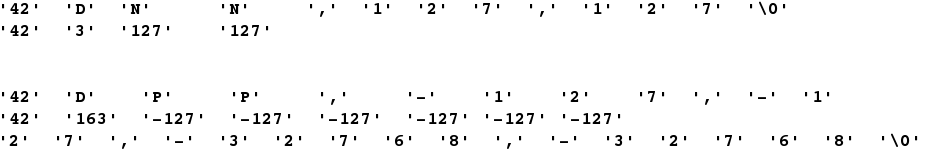
\includegraphics{pictures/vergl_befehle.png}}
 \caption{\label{vergl_befehle}Vergleich von mehreren Befehlen}
\end{figure}
